\section{MatrixRTC}\label{matrixRTC}

Stabilní verze protokolu Matrix podporuje hlasové a video hovory mezi dvěma
uživateli, ale pouze v základní podobě, která nepodporuje skupinové volání,
pozastavování hovorů, renegotiation, algoritmy pro glare resolution,
atp.~\cite{MatrixORG-Spec}.

Kvůli tomu existuje několik MSCs, které navrhují změny specifikace pro přidání
nových funkcí. MSC2746 přidává podporu pro renegotiation, pozastavování hovorů,
upgrady hovorů, restartování ICE, lepší podpora pro více zařízení a
DTMF\footnote{
	\textit{Dual-Tone Multi-Frequency} (\textit{DTMF}) je systém, ve kterém má
	každá číslice přiřazenou dvojici tónů. Tyto tóny se pak používají pro
	komunikaci mezi zařízeními \cite{DSTNY-DTMF}.
} \cite{GitHub-MSC2746}. MSC3077 přidává podporu pro hovory s více streamy
(např. sdílení obrazovek) \cite{GitHub-MSC3077}. MSC3291 pak specifikuje sdílení
metadat o streamech (např. zda je audio či video ztlumené)
\cite{GitHub-MSC3291}.

MSC3401 přidává podporu pro skupinové full-mesh hovory \cite{GitHub-MSC3401}.
MSC3898 pak přidává podporu pro foci (množné číslo od od \textit{focus})
\cite{GitHub-MSC3898}.

\subsection{Využití Matrix primitiv}

Podpora pro VoIP hovory v protokolu Matrix je postavena na již existujících
primitivech. V této části probereme, jak se jednotlivé primitiva využívají.

\subsubsection{Hovory mezi dvěma uživateli}\label{dmCalls}

Hovory mezi dvěma uživateli (stabilní specifikace, MSC2746, MSC3077, MSC3291)
využívají message událostí
\cite{MatrixORG-Spec,GitHub-MSC2746,GitHub-MSC3077,GitHub-MSC3291}.

Typy všech VoIP události mají předponu \mintinline{text}{m.call.} a jejich
\mintinline{text}{content} obsahuje \mintinline{text}{call_id} (unikátní
identifikátor pro daný hovor), \mintinline{text}{party_id} (unikátní
identifikátor pro účastníka hovoru; může být \mintinline{text}{device_id}),
\mintinline{text}{version} (verze VoIP specifikace; měla by být
\mintinline{text}{"1"}) a \mintinline{text}{lifetime} (čas v
\unit{\milli\second}, po který je událost validní)
\cite{MatrixORG-Spec,GitHub-MSC2746}.

Pro zahájení hovoru se využívá událost s typem \mintinline{text}{m.call.invite}.
Její \mintinline{text}{content} obsahuje \mintinline{text}{offer}, která
obsahuje \mintinline{text}{sdp} (SDP offer posílajícího klienta) a
\mintinline{text}{type} (který by měl vždy být \mintinline{text}{"offer"})
\cite{MatrixORG-Spec,GitHub-MSC2746}.

\begin{figure}[H]
	\begin{minted}[tabsize=4,fontsize=\footnotesize]{json}
{
	"type": "m.call.invite",
	"content": {
		"version": "1",
		"call_id": "12345",
		"party_id": "first_party_id",
		"lifetime": 60000,
		"offer": {
			"sdp": "the SDP offer string",
			"type": "offer"
		}
	}
}
	\end{minted}
\end{figure}

Poté, co druhý klient přijme tuto zprávu, by měl poslat na základě rozhodnutí
uživatele buď \mintinline{text}{m.call.answer}, nebo
\mintinline{text}{m.call.reject} \cite{MatrixORG-Spec,GitHub-MSC2746}.

Pokud se uživatel rozhodne hovor přijmout, jeho klient by měl poslat
\mintinline{text}{m.call.answer}, jejíž \mintinline{text}{content} obsahuje
\mintinline{text}{answer}, která obsahuje \mintinline{text}{sdp} (SDP answer) a
\mintinline{text}{type} (který by měl vždy být \mintinline{text}{answer})
\cite{MatrixORG-Spec,GitHub-MSC2746}.

\begin{figure}[H]
	\begin{minted}[tabsize=4,fontsize=\footnotesize]{json}
{
	"type": "m.call.answer",
	"content": {
		"version": "1",
		"call_id": "12345",
		"party_id": "other_party_id",
		"lifetime": 60000,
		"answer": {
			"sdp": "the SDP answer string",
			"type": "answer"
		}
	}
}
	\end{minted}
\end{figure}

Pro předání další ICE kandidátů druhému klientovi je použita událost s~typem
\mintinline{text}{m.call.candidates}, která obsahuje
\mintinline{text}{candidates}, což je seznam ICE kandidátů
\cite{MatrixORG-Spec}. Například JavaScript API pro WebRTC umožňuje kandidáty
konvertovat do JSON pomocí \mintinline{typescript}{RTCIceCandidate::toJSON()}
\cite{MDN-Web-RTCIceCandidate-ToJSON}.

\begin{figure}[H]
	\begin{minted}[tabsize=4,fontsize=\footnotesize]{json}
{
	"type": "m.call.candidates",
	"content": {
		"version": "1",
		"call_id": "12345",
		"party_id": "1355613132",
		"candidates": [
			{
				"candidate": "the candidate string",
				"sdpMLineIndex": 0,
				"sdpMid": "audio"
			}
		]
	}
}
	\end{minted}
\end{figure}

Pokud se uživatel rozhodne hovor odmítnout, jeho klient by měl poslat
\mintinline{text}{m.call.reject} \cite{GitHub-MSC2746}.

\begin{figure}[H]
	\begin{minted}[tabsize=4,fontsize=\footnotesize]{json}
{
	"type": "m.call.reject",
	"content": {
		"version": "1",
		"call_id": "12345",
		"party_id": "1355613132"
	}
}
	\end{minted}
\end{figure}

Je-li při hovoru třeba provést renegotiation, klient by měl poslat s typem
\mintinline{text}{m.call.negotiate}, jejíž \mintinline{text}{content} by měl
obsahovat \mintinline{text}{description} s \mintinline{text}{sdp} (SDP offer
nebo answer) a \mintinline{text}{type} (\mintinline{text}{"offer"} nebo
\mintinline{text}{"answer"}) \cite{GitHub-MSC2746}.

\begin{figure}[H]
	\begin{minted}[tabsize=4,fontsize=\footnotesize]{json}
{
	"type": "m.call.negotiate",
	"content": {
		"version": "1",
		"call_id": "12345",
		"party_id": "1355613132",
		"lifetime": 10000,
		"description": {
			"sdp": "the SDP string",
			"type": "offer"
		}
	}
}
	\end{minted}
\end{figure}

Je-li hovor ukončen, klient by měl poslat událost s typem
\mintinline{text}{m.call.hangup}, jehož \mintinline{text}{content} obsahuje
\mintinline{text}{reason}, která nabývá několika hodnot \cite{GitHub-MSC2746}:
\begin{itemize}
	\itemsep0em
	\item \mintinline{text}{user_hangup} -- uživatel ukončil hovor
	\item \mintinline{text}{invite_timeout} -- druhá strana neodpověděla včas
	\item \mintinline{text}{ice_failed} -- ICE negotiation selhala
	\item \mintinline{text}{ice_timeout} -- spojení selhalo poté, co už byla
	      přeposlána nějaká data
	\item \mintinline{text}{user_media_failed} -- klientovi se nepodařilo získat
	      přístup ke streamu z příslušného zařízení
	\item \mintinline{text}{user_busy} -- primárně pro přemostěné PSTN\footnote{
		      \textit{Public Switched Telephone Network} (\textit{PSTN}) je
		      běžná veřejná telefonní síť \cite{Nextiva-PSTN}.
	      } hovory,
	      kde druhá strana může být nedostupná, protože už s někým telefonuje
	\item \mintinline{text}{unknown_error} -- došlo k neznámé chybě
\end{itemize}

\begin{figure}[H]
	\begin{minted}[tabsize=4,fontsize=\footnotesize]{json}
{
	"type": "m.call.hangup",
	"content": {
		"version": "1",
		"call_id": "12345",
		"party_id": "1355613132",
		"reason": "user_hangup"
	}
}
	\end{minted}
\end{figure}

\subsubsection{Skupinové hovory}

Pro vytvoření skupinového hovoru se využívá \mintinline{text}{m.call} state
událost, jejíž \mintinline{text}{content} obsahuje několik polí
\cite{GitHub-MSC3401}:
\begin{itemize}
	\itemsep0em
	\item \mintinline{text}{m.intent} -- může nabývat několika hodnot
	      \mintinline{text}{m.room} (otevře-li uživatel danou místnost, hovor by měl být
	      jejím hlavním obsahem -- podobně jako Discord voice a video channels), \mintinline{text}{m.prompt} (uživatel by měl být
	      upozorněn, že hovor probíhá), \mintinline{text}{m.ring} (klient uživatele by
	      měl začít vyzvánět)
	\item \mintinline{text}{m.type} -- může být \mintinline{text}{m.voice}, nebo \mintinline{text}{m.video}
	\item \mintinline{text}{m.name} -- libovolný název pro hovor
\end{itemize}

\begin{figure}[H]
	\begin{minted}[tabsize=4,fontsize=\footnotesize]{json}
{
	"type": "m.call",
	"state_key": "cvsiu2893",
	"content": {
		"m.intent": "m.room",
		"m.type": "m.voice",
		"m.name": "Voice room"
	}
}
	\end{minted}
\end{figure}

Chce-li se uživatel připojit do hovoru, pošle \mintinline{text}{m.call.member}
state událost, jejíž \mintinline{text}{content} obsahuje informace o tom, které
zařízení se účastní jakého hovoru \cite{GitHub-MSC3401}. Neobsahuje-li událost
\mintinline{text}{m.foci.} nebo se hovoru účastní jen dva klienti, dojde ke
spojení full-mesh; chování pokud událost tento klíč obsahuje a v hovoru je více
klientů je popsáno v části \ref{foci} \cite{GitHub-MSC3898}. Následně se mezi
jednotlivými zařízeními využívá to-device messages, které jsou ve stejném
formátu jako události popsané v části \ref{dmCalls} \cite{GitHub-MSC3401}.

% MSC3401 dělá velice zvláštní věc, kdy nařizuje max. jeden hovor na místnost,
% ale `m.call.member' event umožňuje se účastnit hovorů více.

\begin{figure}[H]
	\begin{minted}[tabsize=4,fontsize=\footnotesize]{json}
{
	"type": "m.call",
	"state_key": "@user:server.org",
	"content": {
		"m.calls": [
			{
				"m.call_id": "cvsiu2893",
				"m.devices": [
					{
						"device_id": "ASDUHDGFYUW",
						"session_id": "GHKJFKLJLJ",
						"expires_ts": 1654616071686,
						"m.foci.active": [
							{ 
								"user_id": "@sf1:server.org", 
								"device_id": "FS5F589EF" 
							}
						],
						"m.foci.preferred": [
							{ 
								"user_id": "@sfu2:server.org", 
								"device_id": "3FSF589EF" 
							},
							{ 
								"user_id": "@sfu3:server.org", 
								"device_id": "GFSDH93EF" 
							}
						]	
					}
				]
			}
		]
	}
}
	\end{minted}
\end{figure}

\subsection{Klient SDKs}

Aktuálně neexistuje velké množství implementací MatrixRTC, hlavními ale jsou ty,
které si popíšeme v následující sekci.

\subsubsection{Matrix JavaScript SDK}

\href{https://github.com/matrix-org/matrix-js-sdk/}{matrix-js-sdk} je aktuálně
nejvýraznější implementací MatrixRTC s podporou nejvíce funkcí. Podporuje
renegotiation, pozastavování hovorů, upgrady hovorů, restartování ICE, více
zařízení, DTMF, více streamů, sdílení metadat o streamech a skupinové hovory
\cite{GitHub-MatrixJSSDK}. Zároveň se na experimentálním větvi pracuje na
podpoře MSC3898 \cite{GitHub-MatrixJSSDK-MSC3898}.

Element toto SDK využívá na hovory mezi dvěma uživateli a Element Call na
skupinové hovory
\cite{GitHub-ElementCall,GitHub-ElementWeb,GitHub-MatrixReactSDK}.

\subsubsection{Hydrogen SDK}

Další implementací je Hydrogen SDK, které je součástí klient
\href{https://github.com/vector-im/hydrogen-web}{Hydrogen}. Využívá ho právě
klient Hydrogen a Third Room (viz \ref{thirdroom}) \cite{GitHub-Hydrogen}.

\subsection{Foci}\label{foci}

\begin{figure}[H]
	\centering
	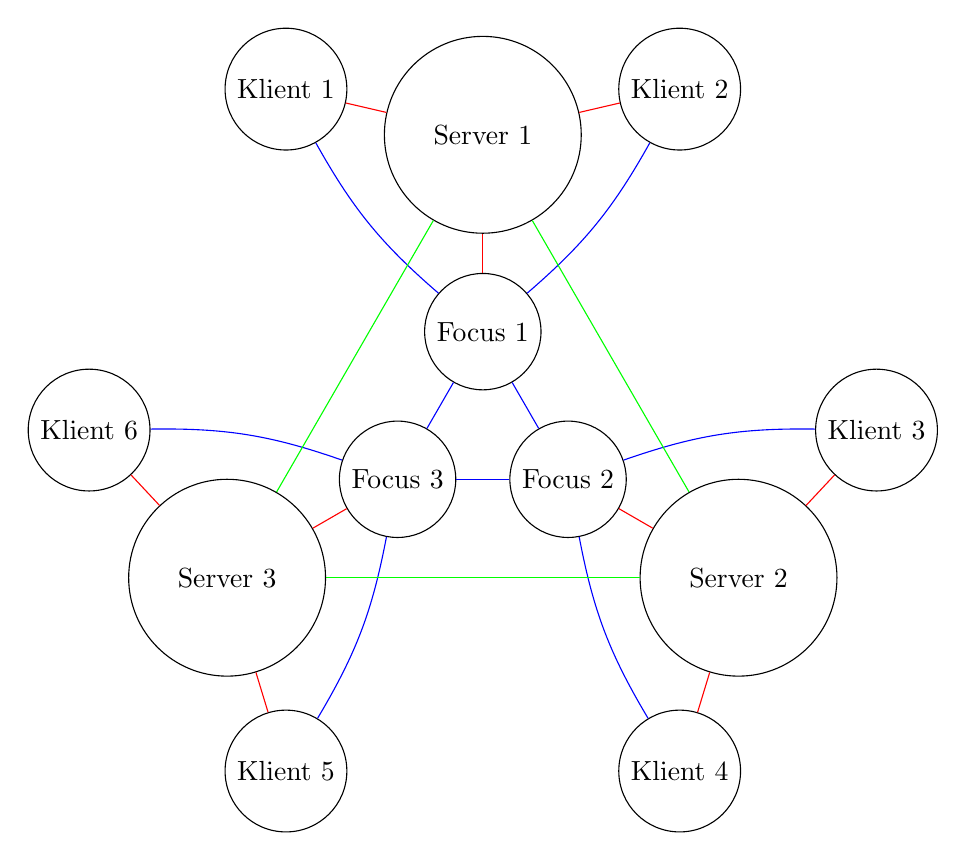
\begin{tikzpicture}[every node/.style={draw,circle}]
		\foreach \i in {1,...,3} {
				\node (focus\i) at ({90-360/3*(\i-1)}:1.25) {Focus \i};
				\node[minimum size=2.5cm] (server\i) at ({90-360/3*(\i-1)}:3.75)
				{Server \i};

				\draw[red] (server\i) -- (focus\i);
			}

		\foreach \i in {1,...,3} {
				\node (client\i) at ({120-360/3*(\i-1)}:5) {Klient {\the\numexpr((\i-1)*2+1)}};

				\draw[red] (server\i) -- (client\i);
				\draw[blue] (focus\i) edge[bend left=10] (client\i);
			}
		\foreach \i in {1,...,3} {
				\node (client{3+\i}) at ({60-360/3*(\i-1)}:5) {Klient {\the\numexpr((\i-1)*2+2)}};

				\draw[red] (server\i) -- (client{3+\i});
				\draw[blue] (focus\i) edge[bend right=10] (client{3+\i});
			}

		\foreach \i in {1,...,2} {
				\foreach \j in {\the\numexpr\i+1,...,3} {
						\draw[green] (server\i) -- (server\j);
						\draw[blue] (focus\i) -- (focus\j);
					}
			}
	\end{tikzpicture}
	\caption{Federace Matrix foci}
	\label{federatedFoci}
\end{figure}

\href{https://github.com/matrix-org/matrix-spec-proposals/pull/3898}{MSC3898}
podporuje tzv. \textit{federované foci}. Na obrázku \ref{federatedFoci} je
vidět, kde jsou federované foci umístěné v Matrix topologii. Jedná se o WebRTC
servery (může se jednat o SFU, MCU či jiný typ serveru), které jsou podobně jako
samotné Matrix homeservery federovány \cite{GitHub-MSC3898}.

\href{https://github.com/matrix-org/matrix-spec-proposals/pull/3898}{MSC3898}
popisuje celý proces výběru a připojování k danému focusu~\cite{GitHub-MSC3898}.
My si situaci vysvětlíme na příkladu.

\begin{figure}[H]
	\centering
	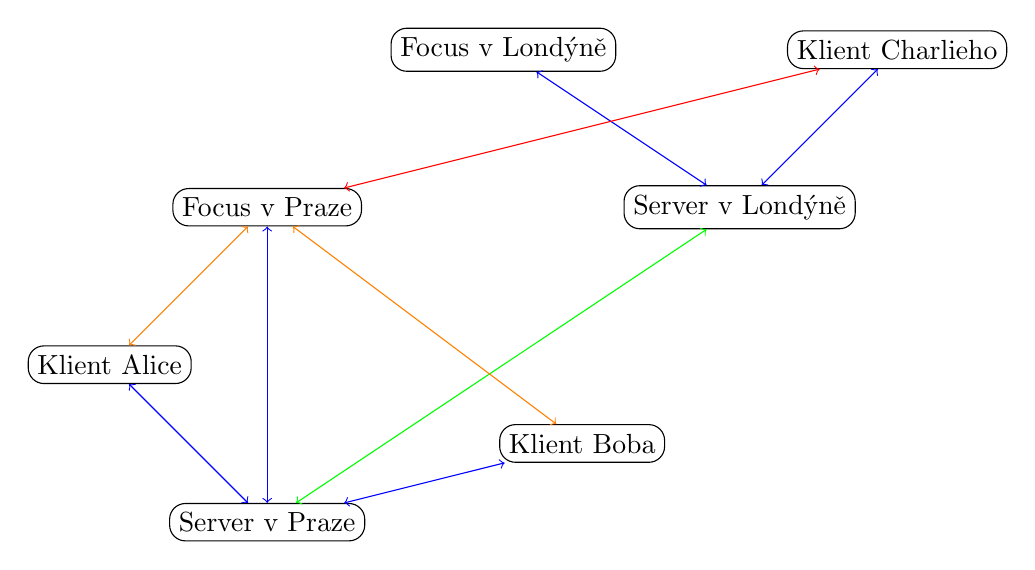
\begin{tikzpicture}[every node/.style={rectangle, rounded corners=2mm}]
		\node[draw] (serverPrague) at (-3,-3) {Server v Praze};
		\node[draw] (serverLondon) at (3,1) {Server v Londýně};

		\node[draw] (focusPrague) at (-3,1) {Focus v Praze};
		\node[draw] (focusLondon) at (0,3) {Focus v Londýně};

		\node[draw] (clientAlice) at (-5,-1) {Klient Alice};
		\node[draw] (clientBob) at (1,-2) {Klient Boba};
		\node[draw] (clientCharlie) at (5,3) {Klient Charlieho};

		\draw[blue, <->] (serverPrague) -- (focusPrague);
		\draw[blue, <->] (serverLondon) -- (focusLondon);

		\draw[green, <->] (serverPrague) -- (serverLondon);

		\draw[orange, <->] (clientAlice) -- (focusPrague);
		\draw[blue, <->] (clientAlice) -- (serverPrague);

		\draw[orange, <->] (clientBob) -- (focusPrague);
		\draw[blue, <->] (clientBob) -- (serverPrague);

		\draw[red, <->] (clientCharlie) -- (focusPrague);
		\draw[blue, <->] (clientCharlie) -- (serverLondon);
	\end{tikzpicture}
	\caption{Federace Matrix foci: Charlie se připojuje do hovoru}
	\label{focusSelection1}
\end{figure}

Na obrázku \ref{focusSelection1} můžeme vidět situaci, kde máme dva Matrix
homeservery (jeden v Praze a druhý v Londýně) a zároveň máme dva Matrix foci
(opět jeden v Praze a druhý v Londýně). Alice a Bob používají pražský homeserver
a jsou připojeni k hovoru, který se aktuálně odehrává na pražském focusu.

Do situace ale vstupuje nový uživatel Charlie, který používá homeserver v
Londýně. Přestože by mohl použít londýnský focus, nepoužije ho a připojí se
rovnou na ten pražský, neboť je aktuálně jediný účastník hovoru z
Londýna~\cite{GitHub-MSC3898}.

\begin{figure}[H]
	\centering
	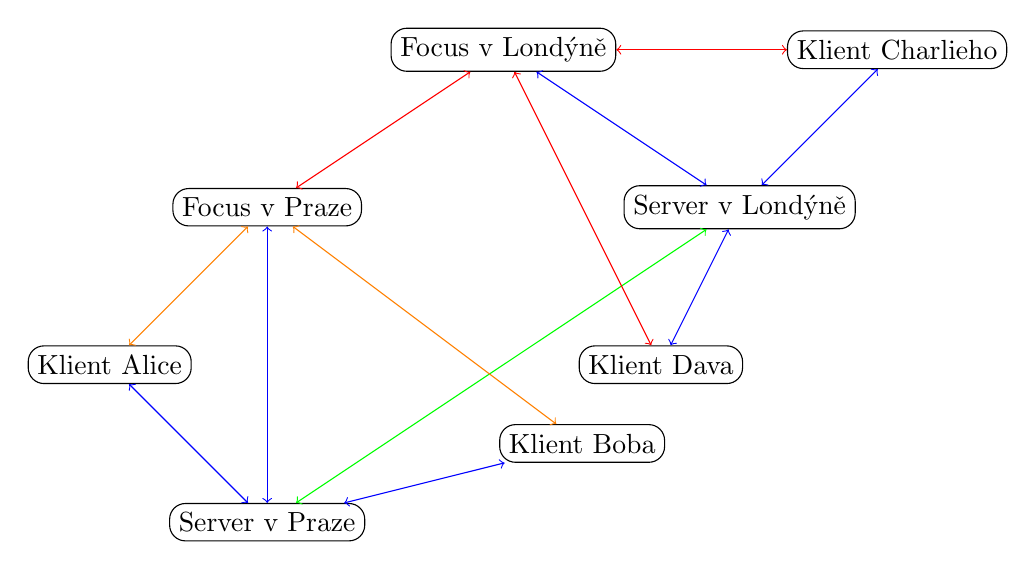
\begin{tikzpicture}[every node/.style={rectangle, rounded corners=2mm}]
		\node[draw] (serverPrague) at (-3,-3) {Server v Praze};
		\node[draw] (serverLondon) at (3,1) {Server v Londýně};

		\node[draw] (focusPrague) at (-3,1) {Focus v Praze};
		\node[draw] (focusLondon) at (0,3) {Focus v Londýně};

		\node[draw] (clientAlice) at (-5,-1) {Klient Alice};
		\node[draw] (clientBob) at (1,-2) {Klient Boba};
		\node[draw] (clientCharlie) at (5,3) {Klient Charlieho};
		\node[draw] (clientDave) at (2,-1) {Klient Dava};

		\draw[blue, <->] (serverPrague) -- (focusPrague);
		\draw[blue, <->] (serverLondon) -- (focusLondon);

		\draw[green, <->] (serverPrague) -- (serverLondon);
		\draw[red, <->] (focusPrague) -- (focusLondon);

		\draw[orange, <->] (clientAlice) -- (focusPrague);
		\draw[blue, <->] (clientAlice) -- (serverPrague);

		\draw[orange, <->] (clientBob) -- (focusPrague);
		\draw[blue, <->] (clientBob) -- (serverPrague);

		\draw[red, <->] (clientCharlie) -- (focusLondon);
		\draw[blue, <->] (clientCharlie) -- (serverLondon);

		\draw[red, <->] (clientDave) -- (focusLondon);
		\draw[blue, <->] (clientDave) -- (serverLondon);
	\end{tikzpicture}
	\caption{Federace Matrix foci: Dave se připojuje do hovoru}
	\label{focusSelection2}
\end{figure}

Na obrázku \ref{focusSelection2} vidíme, že se do hovoru připojil uživatel Dave,
který je podobně jako Charlie v Londýně. Z důvodu, že už máme dva uživatele,
kteří se nacházejí blíže londýnskému focusu, dojde k federaci obou foci
\cite{GitHub-MSC3898}.

\subsubsection{Waterfall}

\href{https://github.com/matrix-org/waterfall/}{Waterfall} je aktuálně jedinou
implementací Matrix focusu. Je napsaná v jazyce Go pomocí knihovny Pion
\cite{GitHub-Waterfall}.
